\chapter{Results \& Discussion}
\label{chapter:results}
\section{Introduction}
The previous chapter discussed an efficient way of finding the contribution of an entire region (\ie complex input feature) with respect to the classification. Building on top of this work, this chapter presents the outcomes of a comprehensive evaluation of the framework proposed in Chapter~\ref{chap:framework}, where the complex input features are selected as described in Chapter~\ref{chap:clustering} and the contribution propagation rules outlined in Chapter~\ref{chapter:REVEAL} are used for assigning a single value of relevance to each complex input feature. The methods proposed in this thesis aim to provide deep insights into the inner workings of models while delivering these insights in an easily graspable manner. To test if the methods provide a interpretable explanations with high fidelity, the explanations are evaluated both qualitatively and quantitatively. 

The novel explainability method is applied on renowned models such as VGG16~\cite{SimonyanZ14a}, VGG19~\cite{SimonyanZ14a}, ResNet50~\cite{he2015deep}, DenseNet121~\cite{huang2018densely} and InceptionV3~\cite{szegedy2015rethinking} and the evaluation is based on the widely recognised ImageNet Large Scale Visual Recognition Challenge 2012 (ILSVRC 2012) dataset~\cite{ILSVRC15}, which has been used in training these models. To facilitate a standardised and consistent analysis, the method described in this chapter is integrated within the iNNvestigate framework~\cite{inn}. This choice not only streamlines the evaluation process but also allows for a comparative analysis with the leading interpretability methods in the field.

In line with standard practices the qualitative analysis compares the \CTC\ method's contribution to classification against established attribution methods, including Input$\times$Gradient~\cite{SimonyanVZ13}, DeconvNet~\cite{ZeilerKTF10}, Guided BackProp~\cite{SpringenbergDBR14}, and LRP-$\alpha_1\beta_0$~\cite{bach2015pixel}. Arguably, showing the single value of \CTC\ makes the comparison between different features and models easier (corroborating results reported in \cite{Ribeiro0G16}). The quantitative analysis is essential to ascertain the relative standing of the \CTC\ method in the context of existing literature, particularly focusing on key interpretability properties such as input invariance and sensitivity, as detailed in Section~\ref{lit:discussion}. The evaluation of these interpretability properties is done by employing fidelity metrics to assess the accuracy of the explainability model. This ensures that the resulting method is not only more interpretable due to the reduced information shown to the user, but also retained the faithfulness of state of the art models.


\section{Qualitative Analysis}

Unique to the approach of selecting complex input features is the visualisation technique employed. It diverges from traditional heatmaps that use seismic colour patterns to represent relevance. Instead, the explanations are assigned a distinct colour to each complex feature's pixels. These colours are then reflected in a colour-coded legend adjacent to the heatmap, clearly illustrating the \CTC\ values and offering a more intuitive understanding of the model's decision-making process.

As the \CTC\ value is assigned to a complex input feature rather than on a pixel level like in other relevance methods, the way the complex input feature is selected influences the results. This chapter presents two ways of selecting the complex input features --- selecting the top features by size, and selecting the top features by the amount of relevance they have received (as described in Chapter~\ref{chap:clustering}). The former doesn't rely on any relevance distribution method to select its features, making it a more independent evaluation and a fairer comparison to other methods in the literature. The latter is particularly useful when there are many features in the input and the relevance serves as a heuristic indicating which ones may be of highest interest to examine. However, due to its dependency on the underlying relevance method for the feature selection, the results are presented separately.  

\subsection{CTC Evaluated Against Different Post-hoc Explanation Methods}

This section focuses on evaluating the performance of the \CTC method on two specific models: VGG16~\cite{SimonyanZ14a} and VGG19~\cite{SimonyanZ14a}. The goal is to compare the explanations generated by the \CTC\ method with those produced by other established post-hoc explanation methods for the same input and models.

\begin{figure}[ht!]
	\begin{center}
		\includegraphics[width=1\linewidth]{Figures/compare_qualitive.pdf}
	\end{center}
	\caption{This figure shows the analysis regarding the predicted class by VGG16~\cite{SimonyanZ14a} as computed by the selected analysers. Each column shows the visualised results for different analysers and each row shows the analyses with respect to the input sample. To the right of the CTC method the value of the contribution of the biggest objects in the input.}
	\label{Fig:quality}
\end{figure} 

Figure~\ref{Fig:quality} provides five examples classified on VGG16~\cite{SimonyanZ14a} and compares the explanations provided by \CTC\ with  Input$\times$Gradient~\cite{SimonyanVZ13}, Integrated Gradients~\cite{SundararajanTY17}, DeconvNet~\cite{ZeilerKTF10}, Guided BackProp~\cite{SpringenbergDBR14}, and LRP-$\alpha_1\beta_0$~\cite{bach2015pixel} methods. The primary advantage of the \CTC\ method lies in its ability to assign a clear, singular value of contribution to the most significant features. Unlike traditional explainability methods, which often yield noisy visual explanations, \CTC\ provides offers a clear and focused perspective on the features deemed most critical by the model.


Arguably \CTC\ not only simplifies the interpretation process but also provides a more accurate representation of what the model deems important. In contrast, earlier methods, while evolving to produce less noisy visual explanations to increase clarity, often overemphasise the importance of edges to the classification. As convolutional layers detect most (if not all edges) it is expected for them to be found relevant. In contrast, \CTC\ delineates a more accurate landscape of feature importance by pinpointing which features truly drive the classification, rather than simply identifying all detectable features. Figure~\ref{Fig:edges} shows three examples, which are classified incorrectly on VGG16 and are explained by Guided Backpropagation, \LRP\ and \CTC.

\begin{figure}[ht!]
	\begin{center}
		\includegraphics[width=0.8\linewidth]{Figures/Edges.pdf}
	\end{center}
	\caption{This figure shows the analysis on the predicted class as computed by the selected analysers. The examples shown were not correctly classified by the VGG16 model.}
	\label{Fig:edges}
\end{figure} 

Established methods do not find it easy to assign relevance to the background, as opposed to the central object and edges in the input. Figure~\ref{Fig:edges} has a set of selected examples, where given the network's classification, the class label is likely driven by the background of the input image rather than the central object. In this example the focus on edges presumably leads to incorrect assumptions. The first input image is of a swimmer next to a pool, which is classified as a ballplayer. Here, \LRP\ provides importance to the majority of edges, while \CTC\ detects the most important feature as being the grass. Similarly, when presented with an input of a framed car, VGG16 classifies the input as a monitor. Guided Backpropagation and \LRP's explanation detects most of the edges and seemingly provide most importance to the car, where as \CTC\ arguably correctly assigns the most importance to the frame itself. The final input is classified as a banister, which is likely due to the pillars at the back rather than the person in the centre of the input. Yet the explanations from Guided Backpropagation and \LRP\ attribute relevance to everything that can be detected. Figure~\ref{Fig:vgg19} provides further examples of the performance of the \CTC\ method compared to the established attribution methods on the VGG19 classifier~\cite{SimonyanZ14a}. 


\begin{figure}[ht!]
	\begin{center}
		\includegraphics[width=1\linewidth]{Figures/compare_qualitive_vgg19.pdf}
	\end{center}
	\caption{This figure shows the analysis regarding the actually predicted class by VGG19~\cite{SimonyanZ14a} as computed by the selected analysers.}
	\label{Fig:vgg19}
\end{figure} 

\subsection{CTC Evaluated on Different Networks}
This section shows the scalability and adaptability of the \CTC\ method across a range of neural network architectures. The diversity in architectural design, exemplified by models such as VGG16~\cite{SimonyanZ14a}, VGG19~\cite{SimonyanZ14a}, ResNet50~\cite{he2015deep}, DenseNet121~\cite{huang2018densely}, and InceptionV3~\cite{szegedy2015rethinking}, presents unique challenges to explainability methods. The goal is to understand how the \CTC\ method performs in different architectural contexts, considering the inherent design and operational differences of these networks. 

Figure~\ref{Fig:compare_models_same} showcases the classification of the same input across various networks, which all correctly classify the input. Crucially, the figure also compares the \CTC method explanation to the established attribution methods.

\begin{figure}[ht!]
	\begin{center}
		\includegraphics[width=1\linewidth]{Figures/methods_differnet_network_same.pdf}
	\end{center}
	\caption{This figure shows the analysis regarding the actually predicted class by different classifier as computed by the selected analysers.}
	\label{Fig:compare_models_same}
\end{figure} 

Figure~\ref{Fig:compare_models_not_same} showcases the classification of the same input across various networks, which are not all classified correctly.

\begin{figure}[ht!]
	\begin{center}
		\includegraphics[width=1\linewidth]{Figures/methods_differnet_network_notsame.pdf}
	\end{center}
	\caption{This figure shows the analysis regarding the actually predicted class by different classifier as computed by the selected analysers.}
	\label{Fig:compare_models_not_same}
\end{figure} 


\subsection{CTC of the Most Relevant Complex Input Features}

This section explores the effectiveness of the \CTC\ method when applied to the most relevant complex input features, as identified by the selection methods in Chapter~\ref{chap:clustering}. By segmenting objects and finding the contribution of the biggest objects one might miss which part of the object makes contributes the most to the classification. Finding small regions of high importance is something state-of-the-art methods excel at. The assignment of contribution to the smaller objects could help the process of pinpointing the exact part of the input that makes an object important.

Figure~\ref{Fig:small_parts} provides examples of the \CTC\ method applied on VGG16, InceptionV3 and ResNet50 where the most relevant complex input feature is selected for relevance distribution.
\begin{figure}[ht!]
	\begin{center}
		\includegraphics[width=1\linewidth]{Figures/relevant_masks.pdf}
	\end{center}
	\caption{This figure shows the CTC value attributed to the most relevant input feature}
	\label{Fig:small_parts}
\end{figure} 



\subsection{Discussion}

\subsubsection{Comparison to other methods}

A critical observation of recent post-hoc explanation methods is the tendency of certain methods, notably Layer-wise Relevance Propagation (LRP), Guided Backpropagation and GradCAM, to disproportionately emphasise the importance of edges in their heatmap representations. This propensity often leads to the overstatement of edges' relevance to the classification decision, potentially obscuring other crucial features. This phenomenon is not merely a visual artefact but a reflection of a deeper interpretative bias within these methods.

This observation aligns with the findings of Adebayo et al.~\cite{AdebayoGMGHK18}, who noted that methods like Guided BackProp~\cite{SpringenbergDBR14} and GradCAM~\cite{ShrikumarGK17} demonstrate a lack of sensitivity to the network's final layers. This insensitivity suggests that these methods are inclined to highlight features such as objects and edges identified by the network's earlier layers, which might not be directly pertinent to the classification's final outcome. 

This is further supported by the results presented in Figure~\ref{Fig:edges}, where LRP and Guided Backpropagation neglect background regions, which may be instrumental in the classification process. This oversight is particularly striking in cases where the background or less prominent features play a key role in the correct classification of the input. For example, in Figure~\ref{Fig:quality}, the bottom image is one of a Chimpanzee playing the piano. One can see that nearly all features (including the piano, a chair, ad other objects in the background) are highlighted by the majority of other methods --- leading the user to assume that nearly all features played a similar role in leading towards the classification. This might lead a user to also assume the network has simply memorised the input, rather than paying much attention to the Chimpanzee. However, this particular image is not part of the ILSVRC 2012 dataset~\cite{ILSVRC15} that the network has been trained on. In contrast \CTC\ presents an ordering of objects and features, and demonstrates that despite the edges of a piano/chair appearing in generic heatmap methods, the most important feature, by several orders of magnitude is the Chimpanzee itself. This is a clear example of the value of \CTC\ in providing a more faithful explanation, and a more interpretable explanation.

This point is perhaps better evidenced in situations of incorrect classification, as shown in Figure~\ref{Fig:edges}. All images have been incorrectly classified, however a generic heatmap does not offer a large amount of information as to \textit{why} this is the case. The tendency of generic heatmap methods to highlight edges and objects, rather than features, means that the user is left with little information as to why the network has made the wrong classification. In contrast, \CTC\ highlights features in the background, or indeed lend relevance to featureless (or edgeless) proportions of the image. An example of this is the background of the Truck/Moniter image in Figure~\ref{Fig:edges}, and on the image of a crib in Figure~\ref{Fig:quality}, which is considerably busy, however a major influence to the network (as found by \CTC) is the blanket. This is hard to spot in a generic heatmap, but the colouring of the blanket is clearly visible in the \CTC\ explanation. Indeed, the feature selection, along with clear ordering of the features provides the user with far clearer and informative explanations.

While conventional methods often struggle to distinctly prioritise the significance of numerous overlapping or closely situated features, the \CTC\ method effectively highlights the most influential features in the classification process. It does so by aggregating and representing the collective importance of feature clusters, thus providing a streamlined and coherent interpretation. By simplifying the complexity inherent in feature-rich inputs, the \CTC\ method unveils the underlying patterns and relationships that may otherwise be obscured in a more granular or dispersed representation. The ability of the \CTC\ method to offer a clear ordering between features is invaluable, especially in scenarios where discerning the relative importance of features is crucial.



\subsubsection{Comparison over different networks}

A critical observation is that the explanations provided by other post-hoc interpretability methods show minimal variation across different networks, rendering it challenging to discern the distinct functional characteristics of each classifier. Furthermore, while LRP-$\alpha_1\beta_0$~\cite{bach2015pixel} generally produces similar explanations across different models, it notably struggles with networks like ResNet50. This inconsistency is likely attributable to the network’s unique structural features, such as residual connections, which impact the method's ability to generate clear explanations.

An interesting facet demonstrated is the effect of network size on the explanations generated. The networks are ordered in Figure~\ref{Fig:compare_models_same} and Figure~\ref{Fig:compare_models_not_same} in ascending order of size, with the smallest network being VGG16, and the deepest with most parameters being DenseNet121. There seems a slight negative correlation between the amount of relevance present in other methods' heatmaps and the network size. This is a pressing problem --- network architectures are tending to grow in size in recent years. \CTC\ demonstrably maintains the amount of information provided to the user. Further, particularly in heatmaps with little information, the segmentation and ordering of relevance of features presents a welcome contrast --- for instance, in Figure~\ref{Fig:compare_models_not_same} the heatmap generated on InceptionV3 is almost entirely blank, with the exception of a small amount of information in the centre of the image. In contrast, \CTC\ extracts an explanation which, in line with \LRP\ and other methods, highlights the head of the water buffalo as the most important feature. However, \CTC\ also highlights the water, and the muddy bank, as being relevant, even if they are of considerably less importance.

The ability of \CTC\ to adapt to larger networks is desired quality, as larger networks, and in particular wider networks, like InceptionV3 are known for memorising components in the training set~\cite{nguyen2020wide}. This is a particular problem in the field of medical imaging, where the training set is often limited, and the network is prone to memorising components of the training set~\cite{alzubaidi2021novel}. A possible example of memorisation is given by the feature-map generated to explain InceptionV3's classification Saluki (a type of dog) in Figure~\ref{Fig:compare_models_same} --- where despite the correct classification being achieved, the most relevant feature is the toy dog/bear next to the Saluki.

In contrast to all other methods explanations, the \CTC\ method's approach to feature ordering provides a more straightforward and insightful analysis. Its ability to distinctly outline and prioritise features makes it easier to identify and understand the differences in the functions learned by various classifiers. This advantage becomes even more pronounced in scenarios depicted in Figure~\ref{Fig:compare_models_not_same}, where inputs are not uniformly classified across all networks. In such cases, an interpretability method like \CTC\ becomes invaluable. It aids in pinpointing differences in the learned functions between correctly and incorrectly classifying networks, offering critical insights into each model's decision-making process.


\subsubsection{Comparison over Relevant Complex Input Features}

A major influence on the quality of \CTC\ heatmaps is the method of feature selection. Most results presented in this chapter demonstrate the selection of masks selected based on size, as opposed to relevance. However, this introduces a bias towards larger features.

Figure~\ref{Fig:small_parts} presents examples of mask selection by a relevance-based ordering. The author suggests this to be the method of choice when applied to complex images with multiple features, wherein the likely cause for a classification is a small, but highly relevant feature. For instance, the top-left hand image of a shoe-store demonstrates a large amount of relevance for a single pair of shoes, which proportionally makes up a very small amount of a feature rich image.

This is further demonstrated by a miss-classification. The second image at the top-left hand of Figure~\ref{Fig:small_parts} presents a photo of a tripod in a chapel, but VGG16 miss-classifies the image as a "swab". When choosing the most relevant complex input features a clear explanation is provided for where the mistake of the reasoning of the classifier lies. A feature selection method with a bias towards larger complex input features, is likely not to have identified this crucial element.

However, this is not always the case. By selecting masks by relevance-based ordering, the shortcomings of other relevance metrics can negatively affect the performance of the \CTC\ explanation generated. For instance, the bottom left image in Figure~\ref{Fig:small_parts} fails to correctly identify the grass-hopper as the major feature in the image, instead showing a preference for smaller features which were attributed a high degree of relevance by the underlying attribution method (\LRP). The explanation in this case is still valid, as these small regions are assigned very low relevance, but it is not explaining which parts do contribute to the classifiers decision. The author suggest that in cases where the most relevant features do not provide an informative explanation the biggest complex input features may provide a better explanation.

% A key strength of the Contribution to Classification (CTC) method becomes apparent in scenarios where inputs possess a high density of features. The CTC method's unique ability to assign a singular relevance value to an entire cluster of features facilitates a clearer and more hierarchically structured interpretation of these features' importance. This aspect of the CTC method is particularly evident when analysing complex inputs, as seen in Figure~\ref{Fig:quality} and Figure~\ref{Fig:vgg19}.

% One of the most significant advantages of the Contribution to Classification (CTC) method is its capability to facilitate clear differentiation and ordered representation of features. This attribute is particularly crucial when analysing and contrasting the performance of different classifiers. In Figure~\ref{Fig:compare_models_same}, the same input is being processed by various networks, all of which correctly classify the input. Here, the figure not only showcases the classifications but also juxtaposes the explanations generated by the CTC method with those from other post-hoc interpretability methods, such as Input$\times$Gradient~\cite{SimonyanVZ13}, DeconvNet~\cite{ZeilerKTF10}, and Guided BackProp~\cite{SpringenbergDBR14}.

% In these figures, we observe inputs processed by the VGG16 model, characterised by their rich feature presence. Here, the CTC method demonstrates its prowess, offering a stark contrast to traditional attribution methods. While conventional methods often struggle to distinctly prioritise the significance of numerous overlapping or closely situated features, the CTC method effectively highlights the most influential features in the classification process. It does so by aggregating and representing the collective importance of feature clusters, thus providing a streamlined and coherent interpretation.


% This clarity in feature prioritisation is not just a matter of visual neatness; it embodies a deeper understanding of the model's decision-making process. By simplifying the complexity inherent in feature-rich inputs, the CTC method unveils the underlying patterns and relationships that may otherwise be obscured in a more granular or dispersed representation. The ability of the CTC method to offer a clear ordering between features is invaluable, especially in scenarios where discerning the relative importance of features is crucial. This characteristic makes the CTC method particularly suited for applications in which a concise yet comprehensive overview of the model's reasoning is necessary.


% A critical observation of recent post-hoc explanation methods is the tendency of certain methods, notably Layer-wise Relevance Propagation (LRP), Guided Backpropagation and GradCAM, to disproportionately emphasise the importance of edges in their heatmap representations. This propensity often leads to the overstatement of edges' relevance to the classification decision, potentially obscuring other crucial features. This phenomenon is not merely a visual artefact but a reflection of a deeper interpretative bias within these methods.

% This observation aligns with the findings of Adebayo et al.~\cite{AdebayoGMGHK18}, who noted that methods like Guided BackProp~\cite{SpringenbergDBR14} and GradCAM~\cite{ShrikumarGK17} demonstrate a lack of sensitivity to the network's final layers. This insensitivity suggests that these methods are inclined to highlight features such as objects and edges identified by the network's earlier layers, which might not be directly pertinent to the classification's final outcome. This is further supported by the results presented in Figure~\ref{Fig:edges}, where LRP and Guided Backpropagation neglect background regions, which may be instrumental in the classification process. This oversight is particularly striking in cases where the background or less prominent features play a key role in the correct classification of the input.

% One of the most significant advantages of the Contribution to Classification (CTC) method is its capability to facilitate clear differentiation and ordered representation of features. This attribute is particularly crucial when analysing and contrasting the performance of different classifiers. In Figure~\ref{Fig:compare_models_same}, the same input is being processed by various networks, all of which correctly classify the input. Here, the figure not only showcases the classifications but also juxtaposes the explanations generated by the CTC method with those from other post-hoc interpretability methods, such as Input$\times$Gradient~\cite{SimonyanVZ13}, DeconvNet~\cite{ZeilerKTF10}, and Guided BackProp~\cite{SpringenbergDBR14}. A critical observation is that the explanations provided by these other methods show minimal variation across different networks, rendering it challenging to discern the distinct functional characteristics of each classifier. Furthermore, while LRP-$\alpha_1\beta_0$~\cite{bach2015pixel} generally produces similar explanations across different models, it notably struggles with networks like ResNet50. This inconsistency is likely attributable to the network’s unique structural features, such as residual connections, which impact the method's ability to generate clear explanations.

% In contrast to all other methods explanations, the CTC method's approach to feature ordering provides a more straightforward and insightful analysis. Its ability to distinctly outline and prioritise features makes it easier to identify and understand the differences in the functions learned by various classifiers. This advantage becomes even more pronounced in scenarios depicted in Figure~\ref{Fig:compare_models_not_same}, where inputs are not uniformly classified across all networks. In such cases, a robust interpretability method like CTC becomes invaluable. It aids in pinpointing differences in the learned functions between correctly and incorrectly classifying networks, offering critical insights into each model's decision-making process.


\section{Quantitative Analysis}
In this subsection, a quantitative analysis is conducted to assess the input invariance and sensitivity of various attribution methods. The focus is on how these methods respond to alterations in the input data, which are introduced to the input through Gaussian noise, Gaussian blurring, and Uniform noise. This evaluation is crucial in determining the robustness of each method against subtle or impactful changes in the input, thereby providing insight into their reliability and consistency in different scenarios. As in the previous section to allow for independent evaluation and fair comparison to other methods in the literature, the contribution is calculated on the biggest masks as identified by SAM.  This is opposed to selecting the masks with the most relevance attributed to them. Given that the change in relevance is what is being measured, the most relevant mask may change, tying the \CTC\ method results with the relevance method used for mask selection. The goal of this analysis is to identify how faithful the \CTC\ rules are by introducing noise to the input, and measuring the variance of the output. Therefore, steps were taken to ensure that any variance in the output is as a result of \CTC\ and the underlying network.


Similarly, the quantitative analysis aims to test the fidelity of the importance value assigned to features, not the clustering technique. To evaluate the \CTC\ value independently of the clustering the biggest masks identified by SAM on the original input are fixed and when evaluated on the noisy inputs. Ultimately, it was decided not to recompute feature-masks for two major reasons: fairness and computational cost. The major consideration is fairness. All other methods have a fixed number of input features, they present one value for each pixel, always evaluated on all pixels, in the case of image classification. As such, it stands to reason that the fairest evaluation method would be to measure the difference in explanations over the same input features --- in other words, were new input features to be computed with each injection of noise, it is not trivial to identify which features have mapped to other features from which to compute the distance. Particularly given that \CTC\ can be employed on top of any existing clustering method, it stands to reasons that fixing masks, and allowing the variance in output to be derived solely from the noise and forward propagation is the most reliable way of assessing the methods robustness and reliability to noise. The second consideration, be it minimal, is that recomputing the feature masks with each introduction of noise would have increased the computational cost of the experiments. While forwards propagation is a relatively cheap operation, the cost of computing the feature masks is not, and would have substantially increased the run-time and cost of the experiments. Particularly given that the results show the evaluation of the \CTC\ method rather than the clustering technique, it was decided that the computational cost exceeded the likely benefits of recomputing feature masks.

\subsection{Input invariance}
\label{input_inv}
Input invariance describes the resilience of an attribution method against certain changes to the input that do not modify the model's output~\cite{YehHSIR19}. Essentially, a robust interpretation method should demonstrate minimal sensitivity to these alterations, meaning it should consistently provide nearly identical explanations even when slight variations are made to the input. To assess the input invariance of the \CTC\ method and how it compares the input invariance of Input$\times$Gradient~\cite{SimonyanVZ13}, Integrated Gradients~\cite{SundararajanTY17}, DeconvNet~\cite{ZeilerKTF10}, Guided BackProp~\cite{SpringenbergDBR14}, and \LRP\-$\alpha_1\beta_0$~\cite{bach2015pixel}, three types of slight variations of the input are introduced.


The first type of input variation is introduced through Gaussian noise using a function that generates noise with a mean of zero and standard deviation of 0.1, which is added to the original image. The second method applies a Gaussian blur, which smooths the image by averaging pixel values in a manner weighted by their proximity to each pixel being processed. The degree of blurring is governed by the size of the Gaussian kernel used in the process, which is $5 \times 5$ in the images generated to test the input invariance of the method. This allows for the blurring to not be too strong. Unlike the Gaussian noise added previously, Gaussian blurring affects the image in a more uniform and systematic way, altering the spatial relationships within the image without introducing extraneous pixel-level variability. The final method introduces Uniform noise. Unlike Gaussian noise, Uniform noise affects all pixels with the same probability and intensity, making it a starkly different test for the attribution method's robustness. The noise is randomly generated within a specified range, which is [-255,255] in the case of images. It is scaled by the intensity parameter, which suits as a noise level. The noise level can hold values between zero and one, where zero means no noise is added to the image and one means that the image is converted only to noise. The noise level parameter was set to 0.02. All resulting noisy images are clipped to ensure all pixel values remain within the [0,255] range, suitable for standard image formats.

\begin{figure}[ht!]
	\begin{center}
		\includegraphics[width=1\linewidth]{Figures/small_noise.pdf}
	\end{center}
	\caption{Examples of images from the ILSVRC 2012 dataset after the introduction of the three types of image alteration --- Gaussian noise addition, Gaussian blurring and Uniform noise.}
	\label{Fig:noisy_images}
\end{figure} 

These three methods of image alteration --- Gaussian noise addition, Gaussian blurring and Uniform noise --- provide distinct challenges to the attribution methods being evaluated. The noise images are generated from the ImageNet Large Scale Visual Recognition Challenge 2012 (ILSVRC 2012) data set~\cite{ILSVRC15} and examples of all three types of noisy images can be seen in Figure~\ref{Fig:noisy_images}. As one may observe, the Gaussian noise introduces pixel-level changes, which are too small for the human eye to notice. The Gaussian blurring alters the image's overall texture and detail and smooths the edges of objects present in the image. Finally, the uniform noise affects all pixels with the same probability and intensity, but as the noise level parameter is quite small it can be mostly observed in the lighter part of images. After generating the modified dataset, explanations were created for each input and its variation --- original, Gaussian blurring, Gaussian noise, and Uniform Noise --- using Input$\times$Gradient, Integrated Gradients, DeconvNet, Guided BackProp, \LRP\-$\alpha_1\beta_0$ and the \CTC\ method. This is followed by a normalisation step before comparing the original and modified inputs, ensuring the sum of explanations equals one. This is especially important for the \CTC\ method, which tends to assign larger values to regions compared to the individual pixel attributions by other methods. The three types of noise present a comprehensive evaluation of how well the \CTC\ method, along with others like Input$\times$Gradient, Integrated Gradients, DeconvNet, Guided BackProp, and \LRP\-$\alpha_1\beta_0$, can maintain consistent interpretations in the presence of subtle input variations. Such resilience is key in ensuring reliable and robust model explanations.


The comparative results, shown in Figure~\ref{Fig:norm}, Figure~\ref{Fig:blur} and Figure~\ref{Fig:uniform}, are based on 500 distinct original inputs. When measuring the input invariance the results show the difference between original inputs explanation and the noisy input explanation only for the noisy images that do \emph{not} change the classification. As input invariance measures the change in explanations when the input has a small change, here if the noisy image changes the classification the noise added is not considered a small change. The distance between the original input's and the noisy input's explanations is calculated using Euclidean distance. Given two $n$-dimensional vectors \( \vec{v}_1 = (v_{1,1}, v_{1,2}, ..., v_{1,n}) \) and \( \vec{v}_2 = (v_{2,1}, v_{2,2}, ..., v_{2,n}) \), where $\vec{v}_1$ is the original image explanations and $ \vec{v}_2$ is the noisy input explanations, the Euclidean distance \( d \) between them is given by:
\begin{equation*}
    d(\vec{v}_1, \vec{v}_2) = \sqrt{\sum_{i=1}^{n} (v_{1,i} - v_{2,i})^2}
\end{equation*}
Here, the summation sums up the squares of the differences of the corresponding components of the two vectors, and the square root is taken of the sum. In all figures the top graph presents the variability of all six methods, bellow a description of each distance vector $\vec{d}$ shows the mean, standard deviation, minimum, 25\%, 50\%, 75\% and the maximum value of each distance vector $\vec{d}$. The bottom left graph shows a zoomed version of all six methods, which ignores the outliers in some methods, such as Guided Backpropagation and makes it easier to see the mean and the standard deviation of the majority of distances. The bottom right graph shows the distances between the original explanations and explanation for the noisy image only for \LRP\ and the \CTC\ methods. As the distance between the original explanations and explanation for the blurry image for those two methods is very small, it is hard to see their mean and standard deviation. This zoomed graph makes it easier to see this information.  

\subsubsection{Gaussian Noise ($\mu = 0, \sigma = 0.1$)}
Figure~\ref{Fig:norm} displays the effects of Gaussian noise. The figure highlights the robustness of specific methods like \LRP\-$\alpha_1\beta_0$ and \CTC, which manage to maintain consistent interpretations in the presence of such noise. Note that out of the 500 inputs this change was tested on 477 noisy inputs which did not result in a change in classification. 
\begin{figure}[ht!]
	\begin{center}
		\includegraphics[width=0.85\linewidth]{Figures/minor_noise_normal_stats.pdf}
	\end{center}
	\caption{The figure highlights how consistent, low-intensity noise, such as the one introduced by the Uniform Noise challenges the robustness of various attribution methods.}
	\label{Fig:norm}
\end{figure} 
\subsubsection{Gaussian Blur ($k = (5 \times 5)$)} The distances between the original explanation and the explanation of the input, which has a small amount of Gaussian blur is shown in Figure~\ref{Fig:blur}. 
\begin{figure}[ht!]
	\begin{center}
		\includegraphics[width=0.85\linewidth]{Figures/minor_blur_stats.pdf}
	\end{center}
	\caption{The figure shows the ability of methods to maintain consistent interpretations in the presence of Gaussian blur.}
	\label{Fig:blur}
\end{figure} 
This blurring, while only subtly altering image details, challenges the attribution methods to maintain accurate interpretations. The figure demonstrates varying degrees of resilience among the methods, with some, like \CTC, effectively preserving their interpretative accuracy despite the blurring. Note that out of the 500 inputs this change was tested on 429, which did not result in a change in classification.
\subsubsection{Small Uniform Noise ($l = 0.02$)}
Figure~\ref{Fig:uniform} focuses on the implications of Uniform noise, which uniformly alters all pixels but with a low intensity, especially affecting lighter image regions. 
\begin{figure}[ht!]
	\begin{center}
		\includegraphics[width=0.85\linewidth]{Figures/minor_noise_uniform_stats.pdf}
	\end{center}
	\caption{The figure highlights how the Uniform Noise challenges the robustness of various attribution methods.}
	\label{Fig:uniform}
\end{figure} 
\newpage
\subsection{Sensitivity}
Sensitivity in interpretability methods refers to how methods react to significant changes in input data. It's crucial that these methods provide distinctly different explanations when the model's classification alters~\cite{NielsenDRRB22}. This section evaluates the sensitivity of the \CTC\ method by comparing it with several other approaches: Input$\times$Gradient~\cite{SimonyanVZ13}, Integrated Gradients~\cite{SundararajanTY17}, DeconvNet~\cite{ZeilerKTF10}, Guided BackProp~\cite{SpringenbergDBR14}, and LRP-$\alpha_1\beta_0$~\cite{bach2015pixel}. To conduct this comparison, the same three significant types of input variations are introduced, but with much higher levels of noise than the ones when testing input invariance.

The first variation adds Gaussian noise with a much higher standard deviation ($\sigma$) than previously used for assessing input invariance. In this case, the standard deviation $\sigma$ is set at 50, compared to the standard deviation of 0.1 used for input invariance evaluation. The second variation creates a blurred version of the original input. The degree of blurring is governed by the size of the Gaussian kernel used in the process, which is $17 \times 17$ for the sensitivity test, in comparison to the $5 \times 5$ Gaussian kernel used for input invariance. The final variation introduces Uniform noise at a level of 0.3, again substantially higher than the 0.02 level used in the input invariance tests. These increased noise levels are designed to rigorously test the sensitivity of the \CTC\ method against state-of-the-art methods. The parameters are set arbitrary to lead to a change in the classification, while still preserving part of the original image.

To visually illustrate the impact of these input variations, Figure \ref{Fig:noisy_images} presents examples of images from the ILSVRC 2012 dataset after the introduction of the three types of significant image alterations. These images serve as a clear representation of the dramatic changes in input data, providing a concrete basis for assessing the sensitivity and robustness of the \CTC\ method in comparison to established techniques. The differences observed in these images are crucial for understanding how each method responds to substantial variations in input. As one may observe, the introduction of blur, Gaussian noise, and Uniform noise to the ILSVRC 2012 dataset images results in significant visual alterations, but the inputs are still somewhat recognisable. After generating the modified dataset, explanations were created for each input image variation --- original, Gaussian noise, Gaussian blurring and Uniform Noise --- using Input$\times$Gradient, Integrated Gradients, DeconvNet, Guided BackProp, LRP-$\alpha_1\beta_0$ and the \CTC\ method.  Similarly to when testing input invariance, the explanations are normalised ensuring the sum of explanations equals one. The three types of noise present a comprehensive evaluation of how well the \CTC\ method, along with others like Input$\times$Gradient, Integrated Gradients, DeconvNet, Guided BackProp, and \LRP\-$\alpha_1\beta_0$, can reflect big changes in the input. Showing a significantly different explanation when the input has been significantly changed is is key in ensuring reliable model explanations. 

\begin{figure}[ht!]
	\begin{center}
		\includegraphics[width=1\linewidth]{Figures/big_noise.pdf}
	\end{center}
	\caption{Examples of images from the ILSVRC 2012 dataset after the introduction of the three types of big image alteration --- Blur ($k = (17 \times 17)$), Gaussian noise addition ($\mu= 0; \sigma=50$) and Uniform noise ($l = 0.3$).}
	\label{Fig:noisy_images}
\end{figure} 

The comparative results, shown in Figure~\ref{Fig:big_gaus}, Figure~\ref{Fig:big_blur} and Figure~\ref{Fig:big_noise_uniform}, are based on the distance between 500 distinct original inputs and their noisy counterparts. As highlighted in Section~\ref{input_inv} certain methodologies exhibit significant alterations in their explanations even with minimal noise introduction. This section aims to evaluate the relative sensitivity of these methods by examining the variance in explanations between examples where noise did not alter the classification and those where it did. This approach allows for an assessment of explanation changes in relation to a baseline alteration for negligible changes. Each figure presents the variability of all six methods between the inputs that changed the classification and the ones that did not. To validate if the difference is statistically significant, a Welch's t-test was performed~\cite{welch1947generalization}. Welch's t-test, also known as the unequal variances t-test, is a statistical test used to compare the means of two groups to determine if they are significantly different from each other. It is an adaptation of the standard Student's t-test~\cite{student1908probable} and is more reliable in real-world scenarios where the assumption of equal variances between groups is often violated.


\subsubsection{Gaussian Noise Addition($\mu = 0, \sigma = 50$)}
The distances between the original explanation and the explanation of the input, which has a big amount of Gaussian Noise added is shown in Figure~\ref{Fig:big_gaus}. This blurring alters image details and should result in attribution methods generating explanations different from the original input.

% Figure~\ref{Fig:noise} displays the effects of Gaussian noise. This type of noise introduces a fine level of randomness, which can potentially mislead attribution methods. The figure highlights the robustness of specific methods like LRP-$\alpha_1\beta_0$ and \CTC, which manage to maintain consistent interpretations in the presence of such noise.

\begin{figure}[ht!]
	\begin{center}
		\includegraphics[width=0.95\linewidth]{Figures/big_gaus.pdf}
	\end{center}
	\caption{The figure shows the challenge big amount of Gaussian noise addition poses to various attribution methods.}
	\label{Fig:big_gaus}
\end{figure} 

\subsubsection{Gaussian Blur ($k = (17 \times 17)$)}
The distances between the original explanation and the explanation of the input, which has a big amount of Gaussian blur is shown in Figure~\ref{Fig:big_blur}. This blurring alters image details and should result in attribution methods generating explanations different from the original input.



% demonstrates varying degrees of resilience among the methods, with some, like \CTC, effectively preserving their interpretative accuracy despite the blurring. Note that out of the 500 inputs this change was tested on 429, which did not result in a change in classification. 
% The top graph 
\begin{figure}[ht!]
	\begin{center}
		\includegraphics[width=0.95\linewidth]{Figures/big_blur.pdf}
	\end{center}
	\caption{The figure shows the challenge a very blurry input poses to various attribution methods.}
	\label{Fig:big_blur}
\end{figure} 

\subsubsection{Uniform Noise Addition($l = 0.3$)}
The distances between the original explanation and the explanation of the input, which has a big amount of Uniform Noise added is shown in Figure~\ref{Fig:big_noise_uniform}. 


\begin{figure}[ht!]
	\begin{center}
		\includegraphics[width=0.95\linewidth]{Figures/big_noise_uniform.pdf}
	\end{center}
	\caption{The figure shows the challenge big amount of Uniform noise addition poses to various attribution methods.}
	\label{Fig:big_noise_uniform}
\end{figure} 

\newpage

\subsection{Discussion}

The key objective of this chapter is to demonstrate that the novel interpretability method, which gives a single value of contribution to the classification (\CTC) to each identified complex input feature, is capable of providing deep insights into the inner workings of models while delivering these insights in an easily graspable manner. A particular concern is that the simplification of evaluating entire features might negatively harm fidelity. To address this, we employed fidelity metrics to compare the performance of \CTC\ against established interpretability techniques. We focused on two essential attributes: \emph{sensitivity} and \emph{input invariance}. Both of these qualities were assessed by introducing noise to the input and observing the resultant variations in the explanations provided. An ideal interpretability method should exhibit low sensitivity to minor noise perturbations, thereby demonstrating input invariance, particularly under the assumption of a robust network. Conversely, a substantial introduction of noise should lead to a noticeable change in explanation. 

The \CTC\ method distinctively assigns a single value to a broad region, inherently minimising its susceptibility to significant changes in response to noise. This stands in marked contrast to other methods, which assign values to individual pixels and, as a result, have a broader scope for discrepancies between the explanations of the original and noise-affected inputs. However, this approach also implies a caveat: if even a small segment of the chosen complex input feature significantly influences the \CTC\ value, it leads to the attribution of an extreme value over a larger area. Such instances can result in notably greater differences in certain explanations compared to other methods, which would only reflect changes in the limited region that has an extreme importance.

Continuing this line of thought, it's noteworthy that overall, the \CTC\ method demonstrates the smallest mean difference between the original and noise-influenced explanations. In some instances, particularly with specific types of noise, this mean difference is over ten times smaller than that of Layer-wise Relevance Propagation (\LRP), which is the second most input invariant method after \CTC. While there is a marginally higher standard deviation observed in \CTC, owing to instances where a small part of a larger feature has a disproportionate impact on the \CTC\ value, these variations remain relatively minimal. The three types of noise and comprehensive evaluation to other methods evidence that the \CTC\ method surpasses others in terms of input invariance, marking it the most stable method in this respect within current literature. 

When accessing the input invariance of the techniques, three types of noise were used: Gaussian noise, small uniform noise, and small blur. The results of only the noisy inputs that did not change the classification are taken. However, the amount of images that did not change the classification was not equal for each type of noise. This indicates that the network is more sensitive to some types of noise than others. In the VGG16 case the biggest impact was seen by small Uniform noise, followed by blurring and Gaussian noise. Further, the impact of the noise to the network could be seen by the change in explanation by \CTC\ and \LRP. The change in explanation was the highest for small uniform noise, followed by blurring and then small Gaussian noise. This was not the case for other methods such as Input $\times$ Gradient, Integrated Gradients, and Guided Backprop and DecovNet. The fact that both \LRP\ and \CTC\ more closely reflect the network's sensitivity to noise further supports the argument that they present more faithful explanations than other methods.


The sensitivity of an interpretability method is assessed by measuring how much its explanation fluctuates with the introduction of noise. This chapter aims to provide a nuanced understanding of these fluctuations. We assess the significance of large changes in explanations by establishing a baseline of minor changes, which serves as a reference point for evaluating the validity of a single explanation. The relevance of a major alteration in the input becomes evident only when contrasted with minor, inconsequential changes. For instance, if an insignificant modification in the input, one that doesn't alter the model's classification, leads to a substantial shift in the explanation, it implies that a major input change would almost certainly result in a significant explanation shift. To contextualise sensitivity, we compare the explanations of inputs with \emph{insignificant} changes --- largest amount of noise that does not affect the classification --- and \emph{significant} changes --- those where the introduced noise does alter the classification, and thus, should also trigger a marked change in the explanation. This approach is part of a broader conversation about the efficacy and intent of these metrics, which is further explored in Chapter~\ref{evl}.

The results clearly indicate that \CTC\ presents a statistically significant change between the explanations with a significant and insignificant noise for all three types of noise presented. Notably, blurring led to the biggest change in input classification. This is expected as it significantly reduces fine details and alters edge information, which are crucial for the network to make it's predictions. In contrast, Gaussian and Uniform Noise tend to add random pixel-level variations that do not fundamentally alter the underlying structures and edges as drastically as blurring does. In this type of noise the integrated gradients and Input $\times$ Gradient were disproportionately effected compared to distance in explanations using Gaussian Noise and Uniform Noise. Gradient methods are sensitive to spatial information and take the gradient with respect to the input. Blurring disrupts the spatial relationships between pixels by averaging them over a region. This smoothing effect can drastically change their explanations, leading to higher sensitivity. As discussed, to evaluate the \CTC\ value independently of the clustering the biggest masks identified by SAM on the original input are fixed and when evaluated on the noisy inputs used without recomputing. This injects more ordered information, as the mask often are dictated by where there used to be edges in the input. The \CTC\ algorithm is therefore less effected by the smoothing operation than Gaussian Noise and Uniform Noise. That being said, it is still statistically different from the inputs that do not change the classification. Further, the \CTC\ method has the second best sensitivity after \LRP\ on inputs with Gaussian Noise and Uniform Noise. 


In summation, it is evident that a quantitative analysis of empirical results demonstrates that \CTC\ exhibits the qualities of sensitivity and input invarience. Indeed, even despite the considerably simplified input, the method demonstrably maintains fidelity to a degree comparable to other leading methods of interpretability. In light of the goals specified by the thesis (simplifying the explanations to reduce the cognitive load upon the explainee while maintaining fidelity), it is fair to conclude that \CTC\ meets the criteria of preserving faithfulness, despite the clear reduction in explanation dimensionality and granularity. Therefore, under the assumption that reducing the number of input features by clustering/segmenting the input space into relevant features does simplify the explanation, the results provide evidence that the research objectives have been met.  


% \section{Conclusion}


    % \item Throughout the results, images were included where the introduction of noise did not result in a change in the classification --- however, one can see that the average change in explanation was \textit{larger} than in comparison to a different type of noise

% \subsection{A meta-analysis of the experimental process}
% There are number of potential reasons why this is a shitty way of evaluating results.
% \begin{itemize}
%     \item Variance/sensitivity of metrics with respect to the size of the features being evaluated. E.g. in the case where there is already noise in the image? 
%     \item When does small noise turn into big noise -- what is the cut-off point where you'd like to see a big change in the explanation as opposed to a small change in the explanation? And how does this relate to the injection of noise? Would the injection of other features make more sense (is it still a ball player if there's an alien and a dog going heels-to-jesus in the background?)
%     \item Variance in the explanations with respect to the variance in the classification perhaps? 
%     \item Distance metrics --- there is some evidence to suggest that the traditional way of measuring distance between two explanations (traditional difference metrics) is not the best way of doing it. E.g. An increase in brightness might be a massive change in euclidean space, but in feature-space, this could be very small. 
%     \item Discussion over the differences between types of noise? We hvae noted that some networks are more sensitive to some types of noise than others. Why would this be the case? 
%     \item Discussion of computational cost in generating explanations? 
% \end{itemize}


% degree of input invariance between \CTC\ and Input$\times$Gradient, Integrated Gradients, DeconvNet, Guided BackProp, and LRP-$\alpha_1\beta_0$. The distance metric used to 


% The 















% employs a function to introduce uniform noise to the images. Unlike Gaussian noise, uniform noise affects all pixels with the same probability and intensity, making it a starkly different test for the attribution method's robustness. The noise is randomly generated within a specified range, which is -255 and 255 in the case of images. It is scaled by the intensity parameter, which suits as a noise level. The noise level can hold values between zero and one, where zero means no noise is added to the image and one means that the image is converted only to noise. The noise level parameter was set to 0.3 The result is then clipped to maintain valid pixel values.



% To asses the input invariance, saturation handling, and sensitivity of the \CTC\ method 

% The 
 

% The \CTC\ value of each complex feature is then found by propagating it through the network starting from the input layer until the classification is reached. We colour all the pixels that belong to each complex feature in one colour and then use that colour in the colour-coded legend next to the heatmap to show the \CTC\ value as a percentage of the overall classification. This deviates from traditional heatmaps, where seismic colours are used to show positive relevance with the intensity of red pixels, and negative relevance with the intensity of blue.
% \begin{figure}[t!]
% 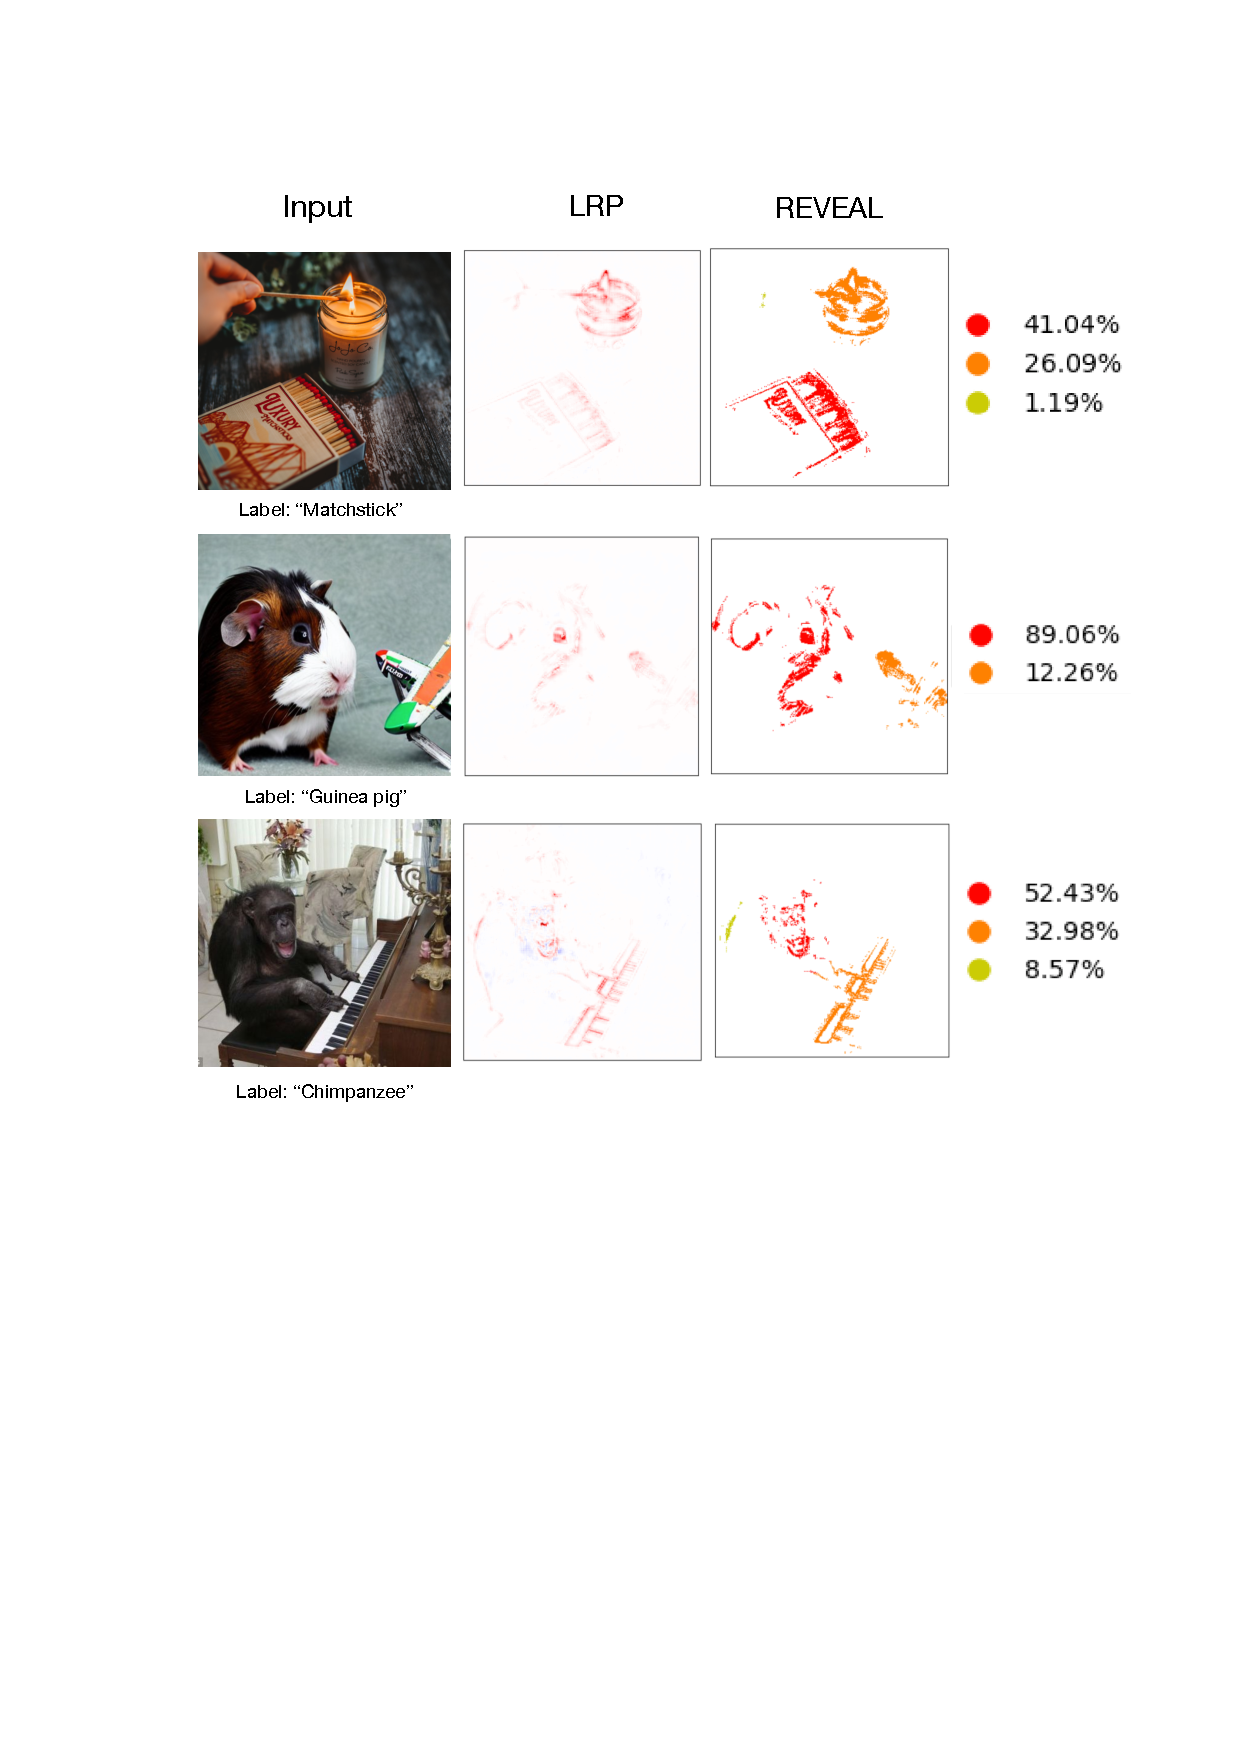
\includegraphics[width=\linewidth]{Chapters/Results/contribution_vs_relevance.pdf}
% 	\caption{Examples showcasing the difference between relevance and the \CTC\ value (contribution) of a feature.}
% 	\label{fig:differnce}
% \end{figure}
% % We argue that the single value of \CTC\ makes the comparison between different features easier. For example in Figure~\ref{fig:all}, when looking at \REVEAL\/'s explanation, each stocking (second row from the top) has a  \CTC\ value in isolation. One in particular (the central stocking) contributes far more than those on either side. This distinction cannot be drawn from any other technique and presents a visible difference even when each stocking is not clearly separated, as when clustering on top of \LRP\/. A similar phenomenon can be seen for the bottom plot of \ref{fig:all}, which is classified as a sports car, with the windscreen seemingly playing an equal part to the front wheel-arch and headlamp in all benchmarks when, in fact, the \CTC\ value is far greater for the wheel -- this is seen when detecting clusters on top of both Input$\times$Gradient and LRP-$\alpha_1\beta_0$.

% In Figure~\ref{fig:differnce} we show more examples that expose the difference between relevance and contribution. We have found that our technique is particularly useful when the input has features that are from two different classes that the network recognises. This brings back the point of relevance based techniques recognising edges that are relevant, but do not contribute much to the classification, as mentioned in section~\ref{subsection:contribution}. In the first example of Figure~\ref{fig:differnce} the classifier labels the input as matchsticks, \LRP\ finds both the matchsticks and the candle relevant, while putting more relevance on the candle. In contrast, \REVEAL\ shows that the matchsticks contribute more to the classification. This can also be seen in third example, where \LRP\ gives almost no relevance to the feature that contributes the most, as presented by \REVEAL\/.  

% The \CTC\ value as a percentage of the overall classification shows us how much of the classification can be explained by the feature alone. Note that the percentages don't total 100\%. As mentioned in Section~\ref{subsection:faithfulness}, this is intentional, as two distinct features may contribute to the same hidden neurons in the network and therefore have an overlapping contribution to the classification.

% As the clusters formed and evaluated by \REVEAL\ are concrete and have a single value of relevance, there is a far smaller chance of inconsistency of the interpretability. This property, as mentioned in section~\ref{subsection:contribution}, requires different users to comprehend the same information from a single explanation. While quantitative analysis is challenging as users find different explanations useful, \REVEAL\ is the only system that has predetermined and quantified complex features making it the only one that achieves that property. 
% \section{Conclusion}
